\documentclass[
    12pt,
    oneside,
    a4paper,
    english,
    brazil
]{abntex2}

\usepackage{lmodern}
\usepackage[T1]{fontenc}
\usepackage[utf8]{inputenc}
\usepackage{indentfirst}
\usepackage{color}
\usepackage{graphicx}
\usepackage{microtype}
\usepackage{amsfonts}
\usepackage{amsmath}
\usepackage{csquotes}

\usepackage{tikz}
\usetikzlibrary{positioning}

\usepackage{caption}

\usepackage[brazilian,hyperpageref]{backref}
\usepackage[alf]{abntex2cite}

\usepackage{macros}

\titulo{Previsão de séries temporais por meio de aprendizado de máquina}
\autor{Guilherme Chichanoski}
\local{Maringá}
\data{2018}
\orientador{Valéria Delisandra Feltrim}
\instituicao{Universidade Estadual de Maringá\\
Centro de Tecnologia --- Departamento de Informática\\
Bacharelado em Ciência da Computação}
\tipotrabalho{Trabalho de Conclusão de Curso}

\preambulo{Trabalho de Conclusão de Curso de Graduação apresentado ao
Departamento de Informática da Universidade Estadual de Maringá, como requisito
parcial para obtenção do grau de Bacharel em Ciência da Computação.}

\makeatletter
\hypersetup{
    pdftitle={\@title},
    pdfauthor={\@author},
    pdfsubject={\imprimirpreambulo},
    pdfcreator={LaTeX with abnTeX2},
    pdfkeywords={séries temporais}{arima}{aprendizado de máquina}{redes neurais},
    colorlinks=true,        % false: boxed links; true: colored links
    linkcolor=red,         % color of internal links
    citecolor=green,         % color of links to bibliography
    filecolor=magenta,      % color of file links
    urlcolor=blue,
    bookmarksdepth=4
}
\makeatother

\setlength{\parindent}{1.3cm}
\setlength{\parskip}{0.2cm}

\begin{document}

\frenchspacing

\imprimircapa{}

\imprimirfolhaderosto{}

\begin{epigrafe}
    \vspace*{\fill}
	\begin{flushright}
		\textit{``Rogo a você que me lê\\
        A sua boa vontade\\
        Não olhe os error, releve,\\
        Guarde com sinceridade\\
        E busque o melhor fazer\\
        Lendo cordel de verdade.''\\
        Raquel Juvêncio e Filomena Mourão}
	\end{flushright}
\end{epigrafe}

\begin{resumo}
    % TODO: Resumo

    \textbf{Palavras-chave}: séries temporais, arima, aprendizado de máquina,
    redes neurais.
\end{resumo}

\begin{resumo}[Abstract]
    \begin{otherlanguage*}{english}
        % TODO: Abstract

        \textbf{Keywords}: time series, arima, machine learning, neural
        networks.
    \end{otherlanguage*}
\end{resumo}

\textual{}

\pdfbookmark[0]{\contentsname}{toc}
\tableofcontents*
\cleardoublepage{}

\chapter{Introdução}

%VALERIA: Evite usar a 1a pessoa no texto ("podemos..., fizemos...", etc.). Embora essa forma seja comum na escrita científica em inglês, em português não é usual. Eu já corrigi essa questão em toda a parte revisada (até o início dos modelos probabilísticos). Por favor, corrija no restante.

Segundo \citeonline{wiley} prever é a capacidade de predizer valores ou eventos
futuros e  constitui uma  tarefa de grande  importância para  diversos setores,
incluindo governos e industrias. Uma vez  que tal capacidade é parte crucial na
tomada de decisão,  fica evidente a necessidade de se  realizar boas previsões.
No entanto,  fazer boas  previsões pode ser  uma tarefa  extremamente complexa.
Muitos autores  e organizações já realizaram  previsões que, com o  decorrer do
tempo, se mostraram erradas, como no caso  do The New York Times, que previu em
1966  que existiriam  somente 220.000  computadores nos  Estados Unidos  no ano
2000.

Ainda conforme  \citeonline{wiley}, as  previsões são classificadas  como sendo
de  curto,  médio  e  longo  prazo,   sendo  o  prazo  definido  na  frequência
das  observações.  Quando denominadas  de  curto  prazo, são  previstas  poucas
observações  a frente  do tempo  atual. Já  previsões de  médio prazo  podem se
estender por algumas observações no futuro.  Por fim, previsões que envolvem um
período maior  no futuro são chamadas  de longo prazo. Ainda  conforme o autor,
predições de médio e longo prazo são mais difíceis de se realizar e suscetíveis
a fatores externos.

% FIXME Acredito que deveria estar nos trabalhos relacionados
%Em  \citeonline{giebel2011state} o  autor  realiza a  predição  da geração  de
%energia eólica, a produção é dada em função da capacidade na região instalada,
%o vento,  no entanto, é  um elemento volátil  e sendo assim  existirá momentos
%quais o  uso de outras  fontes será necessária,  contudo, é preciso  ter certo
%conhecimento prévio,  pois, o ligamento  de uma  usina como aquelas  movidas a
%gasóleo podem levar até  duas horas. Logo prever duas horas  a frente pode ser
%crucial  para  garantir o  abastecimento  de  energia  a uma  região,  podendo
%impactar no cotidiano e economia de uma população.

Para a realização da previsão é necessária  a compreensão do evento que se quer
prever. Quando  existe uma relação temporal  entre as observações do  evento em
questão,  i.e., o  evento  ocorre  em uma  determinada  sequência  no tempo,  é
necessário organizar  as informações  de forma a  evidenciar a  dependência das
observações com  seus estados anteriores.  Nesse caso, as  observações passadas
compõem uma  série temporal, a  partir da qual  é possível realizar  medições e
produzir modelos capazes de expressar  matematicamente o comportamento da série
em  função de  suas  observações  anteriores, permitindo  assim  a predição  de
estados futuros.


% FIXME: Tá esquisito 
% VALERIA: não está claro o que vc quer  mostrar com essa figura! O que vc quer
% que o  leitor observe?  Além disso, vc  precisa dizer  o que os  eixos x  e y
% significam.
Conforme  mencionado,   as  séries  temporais  são   compostas  de  observações
sequenciais ao  longo do  tempo~\cite{wiley}. Como exemplo,  a \autoref{serie0}
mostra uma série gerada utilizando-se um processo de caminhada aleatória. Sendo
essas observações  separadas unicamente pelo  tempo, pode-se obter os  dados em
diferentes intervalos, como observações diárias, semanais ou anuais.
% VALERIA: Arrumei a escrita, mas veja se é isso mesmo que vc queria dizer
Conforme \citeonline{ehlers},  devido à caraterística estocástica  do processo,
uma observação se define em função de suas antecessoras.

\begin{figure}[ht]
    \centering
    \caption{Série gerada para exemplo}\label{serie0}
    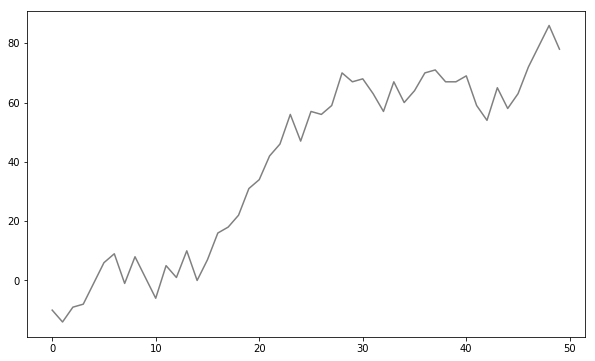
\includegraphics[width=.6\linewidth]{images/serie_exemplo.png}
    \source{Elaborado pelo autor}
\end{figure}

Considerando  então  que  a  série  apresentará  comportamento  estocástico,  é
possível  propor  modelos  que  serão  capazes  de  aproximar  o  comportamento
da  série.  Os  modelos  comumente  utilizados para  essa  tarefa  são  aqueles
probabilísticos, mais especificamente o ARIMA\@, proposto por \citeonline{box}.
Também é possível utilizar modelos criados a partir da aplicação de técnicas de
aprendizado de máquina,  que vem se apresentando como  uma alternativa poderosa
em muitas aplicações.

Com o  constante interesse na  aplicação e  a identificação das  capacidades de
técnicas de  aprendizado, fica  evidente a importância  de observar  como esses
modelos se comparam com os estatísticos. Dessa forma, o objetivo deste trabalho
foi comparar o desempenho de modelos  estatísticos e baseados em aprendizado de
máquina na previsão de uma  série de característica econômica. Especificamente,
foram  avaliados  o  modelo  estatístico  ARIMA  e  um  modelo  de  aprendizado
de  máquina baseado  em  redes  neurais artificiais  de  múltiplas camadas.  Os
resultados indicaram  que os modelos  tiveram desempenho semelhantes  nos dados
utilizados nesse trabalho.

% Como  forma de  comparar desempenhos  e  buscar compreender  as técnicas  que
% poderiam ser utilizadas para a previsão, este trabalho realizou a previsão de
% uma série de característica econômica utilizando ambas metodologias.

% TODO: Introduzir modelos ARIMA com exemplos de artigos

% FIXME Mais adequado na parte de trabalhos relacionados
%vez mais  notórias pelos bons resultados  que oferecem. \citeonline{artigoEx3}
%Em contrapartida, técnicas  de aprendizado de máquinas estão  se tornando cada
%aplicou  métodos  de aprendizado  de  máquina  possibilitando a  previsão  com
%bons  resultados. Pelo  fato  dos modelos  estatísticos fornecerem  resultados
%satisfatórios para predições e estarem bem difundidos na comunidade acadêmica,
%é  comum  que  trabalhos  como \citeonline{artigoEx4}  compare  os  resultados
%obtidos  a  partir  de  aprendizado   de  máquina  com  modelos  de  abordagem
%estatísticas. Para modelos de aprendizado se  destaca aqueles com uso de redes
%neurais  artificiais  por serem  capazes  de  obter bons  resultados  conforme
%analisado  por \citeonline{zhang},  o  autor ainda  apresenta outros  exemplos
%quais os autores obtiveram resultados superiores ao método estatístico.

O    restante   desta    monografia    está   organizada    como   segue.    No
\autoref{chap:fundTeor}  é apresentada  a  fundamentação  teórica do  trabalho,
incluindo os principais métodos de  previsão de séries temporais empregados. No
\autoref{chap:desenv} são  descritos os passos metodológicos  empregados para a
desenvolvimento tanto do  modelo estatístico quanto de  aprendizado de máquina.
Os  resultados obtidos  com base  nos modelos  construídos são  apresentados no
\autoref{chap:result} e  apresentada as  constatações feitas em  ambos modelos.
Por  fim,  no  \autoref{chap:concl}  é  apresentada  a  conclusão  do  que  foi
realizado.

\chapter{Fundamentação teórica}\label{chap:fundTeor}

\section{Previsão}
Segundo  \citeonline{wiley},  o  processo  de previsão  pode  ser  dividido  em
diversas atividades, dispostas a seguir:

\begin{enumerate}
    \item Definição do problema\\
        Envolve  definir e  entender  a  tarefa de  previsão  a ser  realizada,
        considerando o prazo a ser previsto e definindo os dados necessários.
    \item Coleta dos dados\\
        Envolve a coleta  dos dados necessários de acordo com  as definições da
        atividade anterior.
    \item Análise dos dados\\
        Atividade de alta  importância para a seleção do  modelo mais adequado.
        Nessa  etapa   são  utilizadas  observações  gráficas   e  extração  de
        características para identificar padrões  que corroborem na escolha dos
        parâmetros. Também são identificadas  observações problemáticas e, caso
        necessário, aplicadas as devidas correções.
    \item Seleção e verificação do modelo\\
        A partir  da análise  feita na atividade  anterior, será  selecionado o
        modelo, analisando-se  também o comportamento com  os dados fornecidos.
        Como  método de  verificação são  utilizadas métricas  que favoreçam  a
        comparação.
    \item Avaliação do modelo\\
        Atividade na qual se avalia como  o modelo se comporta com novos dados,
        normalmente realizada  com observações  excluídas dos  dados utilizados
        nas atividades anteriores. As  observações separadas para avaliação são
        utilizadas apenas para essa finalidade.
    \item Publicação do modelo\\
        Com o modelo devidamente selecionado e avaliado, o mesmo é instalado em
        ambiente de produção, observando-se  as alterações necessárias para que
        novos dados sejam inseridos corretamente.
    \item Monitoramento do desempenho do modelo\\
        Deve-se continuamente  avaliar como  o modelo  aplicado se  comporta em
        relação ao ambiente, já que o ambiente é algo volátil.
\end{enumerate}

Essas  atividades normalmente  são realizadas  em ordem  semelhante a  exposta.
Vale  observar ainda  que  se os  resultados da  atividade  de avaliação  forem
insatisfatórios, deve-se  retornar à atividade  anterior e refazer  a avaliação
até que um modelo que obedeça às especificações seja encontrado.

\section{Séries temporais}\label{sec:seriesTemporais}

Como  exposto anteriormente,  séries  temporais são  compostas por  observações
sucessivas  feitas ao  longo do  tempo. Cabe  destacar ainda  que essas  séries
se  caracterizam   pelo  fato  de   suas  observações  serem   dependentes  das
observações  anteriores. Além  disso,  tais  séries demonstram  características
como  tendência e  sazonalidade.  A tendência  caracteriza  o comportamento  de
crescimento/decrescimento da série, o que  pode levar a observações futuras com
valores  menores ou  maiores. A  sazonalidade caracteriza  padrões cíclicos  em
função do tempo, comumente tomando períodos semanais, mensais ou anuais.

Uma série é descrita matematicamente pelo conjunto $\{X(t): t \in T\}$, podendo
$t$ ser  um tempo  contínuo ou  discreto. O  tempo $t$  é dito  contínuo quando
se  possui  observações  $X(t)$  para  todo $t$  em  $T$,  sendo  $T  \subseteq
\mathbb{R}^{+}$. O tempo $t$ é discreto  quando entre as observações $X(t_i)$ e
$X(t_{i+1})$ existe um  intervalo igual de tempo, normalmente dado  na forma de
uma sequência, $T = \{1, 2, \ldots, n\}$, sendo $n$ o número de observações.

Segundo  \citeonline{ehlers}, uma  série  temporal  classicamente é  decomposta
seguindo a \autoref{eq:timeseries}, sendo $t$ usado para denotar o tempo, logo,
é parte fundamental entender o comportamento segundo essas três componentes.

\begin{equation}
    \label{eq:timeseries}
    X_t = Tendência_t + Sazonal_t + Aleatório_t
\end{equation}

\subsection{Série estacionária}

%VALERIA: tirei essa definição de um site de estatística
%http://www.portalaction.com.br/series-temporais/13-processos-estacionarios
% mas precisaria usar uma definição tirada de um livro.
Um  conceito importante  para a  análise de  séries temporais  é o  seu caráter
estacionário. Um processo é dito  estacionário se todas as suas características
comportamentais  não se  alteram  ao  longo do  tempo.  Em  outras palavras,  o
processo se desenvolve no tempo em torno da média, de modo que a escolha de uma
origem dos  tempos não é  importante. Segundo \citeonline{ehlers}, uma  série é
dita estritamente estacionária quando  a distribuição de probabilidade conjunta
de  $X(t_1), \ldots,  X(t_k)$ é  igual a  de $X(t_1  + \tau),  \ldots, X(t_k  +
\tau)$.

Ainda segundo \citeonline{ehlers}, a definição  estrita de série estacionária é
dificilmente  aplicada,  então  usualmente  se utiliza  a  definição  de  série
fracamente estacionária,  que se define com  base no critério da  mesma possuir
função média  constante. Dessa forma,  no decorrer  deste trabalho, se  usará a
definição  de  série fracamente  estacionária  para  se  tomar uma  série  como
estacionária.

Em  termos matemáticos,  usa-se a  \autoref{eq:westacionaria} para  definir que
variância  de um  elemento da  série ($z_t$)  deve ser  semelhante à  média. Em
outras  palavras, o  deslocamento da  origem do  tempo $t$  por uma  quantidade
$\tau$ não  exerce efeito  na distribuição  conjunta da  série. Assim,  o valor
esperado para a série em determinado momento não será dada em função do tempo.

\begin{equation}
    \label{eq:westacionaria}
    E(z_t) = \mu_t = \mu
\end{equation}

% FIXME Dada em função de que??


%TODO Adicionar referência ao Livro Time Series by exmples

%TODO Adicionar referência ao teste de Dockey Fuller

% VALERIA: Deixe para mostrar o exemplo da série estacionária pós-diferenciação
% na seção que fala  sobre a diferenciação. Neste ponto do  texto ficou fora de
% contexto. Ou, se  vc quer mostrar um exemplo, mostre  uma série originalmente
% estacionária. Além  disso, nesse caso, vc  tem que explicar melhor  a figura.
% Por exemplo,  qual(is) característica(s) do  gráfico da série me  diz(em) que
% ela é  estacionária? Dizer  que a  observação do gráfico  é suficiente  não é
% suficiente. ;)

A  \autoref{fig:co2diff}   é  um  exemplo  de   série  estacionária  encontrada
ao   aplicar   o   processo   de  diferenciação   na   série   apresentada   na
\autoref{fig:co2}, este  processo está descrito na  \autoref{sec:diff}. Segundo
\citeonline{tsExample} embora  exista testes  como o  de Dikey  Fuller descrito
em  \citeonline{dickey}  para  a  prova de  estacionariedade,  é  suficiente  a
observação  gráfica  da  série.  Mas  caso não  seja  conclusiva  a  observação
\citeonline{tsExample} orienta obter  o gráfico da função  de autocorrelação, e
se  observada a  existência de  mais de  20 correlações  significativas pode-se
classificar a série como não estacionaria.

\subsection{Sazonalidade e tendência}

Conforme   definido  por   \citeonline{ehlers},   a  sazonalidade   caracteriza
repetições de comportamento de uma série em um período $s$ de tempo. A presença
da sazonalidade, em  geral, é facilmente observada na  representação gráfica da
série, conforme exemplificado no gráfico  da \autoref{fig:co2}. Nesse gráfico é
apresentada uma série  temporal real que registra a mudança  na concentração de
$CO_2$ na atmosfera. Observando o gráfico, é possível notar que há sazonalidade
de periodicidade anual, devido ao gráfico apresentar formato de serra e está se
apresentar em repetição anual.

Ainda  no  gráfico  da  \autoref{fig:co2},  também  é  possível  notar  que  há
uma  tendência de  crescimento na  série. Segundo  \citeonline{ehlers}, não  há
uma  definição exata  de  tendência, mas  normalmente a  mesma  é associada  ao
comportamento  de  mudança  das  observações  ao longo  de  um  vasto  período.
Uma  série  com tendência  pode  ser  descrita  como  a função  apresentada  na
\autoref{eq:tendencia},  na  qual $\alpha$  e  $\beta$  são os  coeficientes  e
$\epsilon_t$ é  o erro. O coeficiente  $\beta$ define a taxa  de crescimento da
série  e, desse  modo, $\beta$  pode  ser entendido  na  forma $\beta  = x_t  -
x_{t-1}$.

\begin{equation}
    \label{eq:tendencia} X_t = \alpha + \beta_t + \epsilon_t
\end{equation}

Esse entendimento de série  com tendência, segundo \citeonline{ehlers}, permite
encontrar uma  função polinomial representativa  da série na forma  mostrada na
\autoref{eq:tendenciaSerie}.

\begin{equation}
    \label{eq:tendenciaSerie}
    X_t = \beta_0 + \beta_1t + \beta_2t^2 + \cdots + \beta_{p}t^p + \epsilon_t
\end{equation}

% Um exemplo real de uma série  temporal que apresenta tendência e sazonalidade
% é mostrado  no gráfico  na \autoref{fig:co2}. Essa  série registra  a mudança
% na  concentração  de $CO_2$  na  atmosfera,  sendo,  portanto, uma  série  de
% característica natural.  Observando o gráfico,  é fácil notar a  tendência de
% crescimento da série e sua sazonalidade de periodicidade anual.

\begin{figure}
    \centering
    \caption{Leituras de $CO_2$ na atmosfera.}\label{fig:co2}
    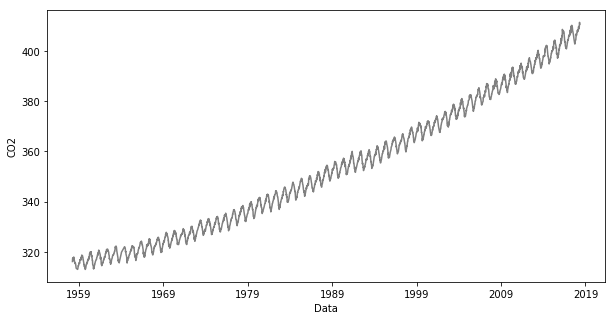
\includegraphics[width=.6\linewidth]{images/co2.png}
    \source{\citeonline{co2data}}
\end{figure}

\subsubsection{Filtros}

%VALERIA:essas flutuações seriam a sazonalidade?
Em algumas séries a tendência pode  não estar evidente devido a flutuações. Por
conta disso, pode  ser necessária a aplicação de filtros  que têm como objetivo
obter  uma série  suavizada que  possibilite  observar a  tendência. Um  desses
filtros é apresentado na \autoref{eq:filtro} \cite{ehlers}.

\begin{equation}
    \label{eq:filtro}
    y_t = \sum_{j = -q}^{s}{a_{j}x_{t+j}}
\end{equation}

%VALERIA:  Cada termo  da soma  é uma  observação? Se  for, não  ficaria melhor
%dizer: $a_j$  é um  peso aplicado  a cada observação  da série,  observado que
%$\sum{a_j} = 1$? Também precisa dizer o que é o 't', o 'q' e o 's'
Na \autoref{eq:filtro}, $a_j$  é um coeficiente a ser aplicado  a cada termo da
soma de forma a aplicar um peso a este, sendo observado que $\sum{a_j} = 1$.
%VALERIA: Qual é o caso mais simples?
Podemos obter, no caso  mais simples, $a_j = \frac{1}{2q +  1}$ e teremos $y_j$
conforme a \autoref{eq:yjfiltro}.

\begin{equation}
    \label{eq:yjfiltro}
    y_t = \frac{1}{2q + 1}\sum_{j=-q}^{q}{x_{t+j}}
\end{equation}

A \autoref{eq:yjfiltro} é conhecida por fornecer o cálculo das médias móveis.
% VALERIA: se  o filtro  de médias  móveis serve  para remover  a sazonalidade,
% precisa dizer antes de comentar sobre o gráfico.
A aplicação do filtro de médias móveis  na série das leituras de $CO_2$ resulta
na \autoref{fig:co2filtrado},  que evidencia de forma  independente a tendência
da série após a remoção da sazonalidade.

\begin{figure}
    \centering
    \caption{Leituras de $CO_2$ filtrada utilizando médias móveis com $q$ igual
        a $52$, devido à sazonalidade ser anual, ou seja, $52$
        semanas.}\label{fig:co2filtrado}
    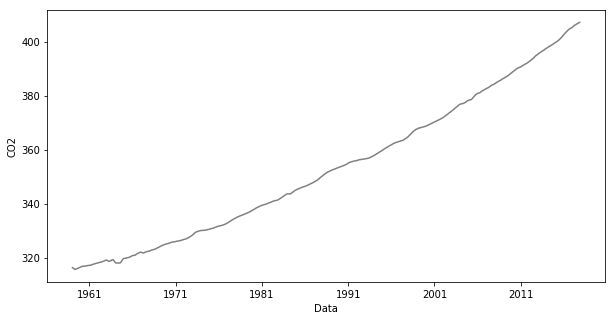
\includegraphics[width=.6\linewidth]{images/co2_filtered.png}
    \source{Elaborado pelo próprio autor a partir de \citeonline{co2data}}
\end{figure}

\subsubsection{Diferenciação}\label{sec:diff}

Outra tarefa a ser observada em relação  ao entendimento de tendência é a forma
na qual é removida. O método mais  simples para remoção da tendência é subtrair
de  cada valor  observado  o  valor do  seu  antecessor,  conforme descrito  na
\autoref{eq:diferenciacao}. Normalmente,  uma única diferenciação  é suficiente
para remover  a tendência, porém em  séries com componente sazonal  podem vir a
ser necessárias mais de uma em um \textit{lag} diferente.

\begin{equation}
    \label{eq:diferenciacao}
    y_t = x_t - x_{t-1}
\end{equation}


O gráfico  da \autoref{fig:co2diff} mostra o  resultado obtido para a  série de
leituras de $CO_2$ após uma diferenciação.
%VALERIA: vc começou dizendo que a diferenciação serve para remover tendência e concluiu dizendo que a diferenciação evidenciou a componente sazonal (?!). Qual a relação? Além disso, por que esse gráfico evidencia a componente sazonal? Explique isso ao leitor.
Pelo gráfico  é possível  perceber que  a série resultante  se aproxima  de uma
série com função média constante, dando evidência a componente sazonal.

Para  dar  um   exemplo  de  diferenciação  volto  a  série   das  leituras  do
$CO_2$  e  agora   realizando  uma  diferenciação,  o  resultado   é  visto  na
\autoref{fig:co2diff}, especificamente neste exemplo  percebemos que a série se
aproximou de  uma série  com função  média constante,  dando ainda  evidência a
componente sazonal.

\begin{figure}
    \centering
    \caption{Série da leitura do $CO_2$ na atmosfera com uma
        diferenciação}\label{fig:co2diff}
    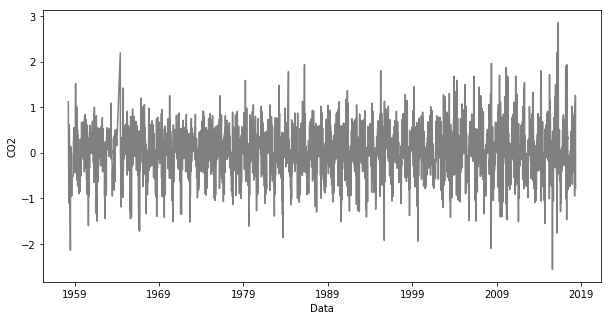
\includegraphics[width=.6\linewidth]{images/co2_diff.png}
    \source{Elaborado pelo autor a partir de \citeonline{co2data}}
\end{figure}

% \subsection{Sazonalidade}

% Conforme definido por \citeonline{ehlers} sazonalidade caracteriza repetições
% de comportamento de uma série em um período $s$ de tempo. Normalmente é
% facilmente observado na representação gráfica da série.

\section{Modelos probabilísticos}

Conforme  apresentado anteriormente,  as séries  temporais podem  ser previstas
utilizando-se modelos  estatísticos. Segundo \citeonline{ehlers}, isso  se deve
ao  seu caráter  estocástico, uma  vez  que cada  observação possui  correlação
com  as  observações  imediatamente   antecessoras,  diferentemente  de  séries
determinísticas, as quais têm seu estado  definido por uma função matemática ou
um sistema para o qual a saída é dependente apenas das entradas atuais.

Um modelo comumente utilizado para a  previsão de séries temporais é o ARIMA\@.
Descrito por  \citeonline{box}, esse  modelo caracteriza a  série em  termos de
três  parâmetros $(p,d,q)$,  sendo  cada  um associado  a  um  processo: $p$  é
associado a  processos auto-regressivos, $r$  a processos integrativos e  $q$ a
processos de médias móveis.

A  definição dos  valores  desses parâmetros  não  é direta  e  depende de  uma
análise  das  características  da  série.  \citeonline{box}  descreveu  algumas
ferramentas que podem auxiliar nessa análise, entre elas a análise da função de
autocorrelação.

\subsection{Função de autocorrelação}\label{sec:corre}

%Conforme mencionado, a análise da função de correlação é uma ferramenta que auxilia na identificação do comportamento da série \cite{box}.
%, uma ferramenta para isso é a função de autocorrelação, 
%VALERIA: a definição abaixo ficou "solta"
%Com base na correlação entre duas séries $X$ e $Y$, é possível obter a correlação de uma série com defasagem $k$, sendo essa defasagem a distância entre o valor analisado $X_t$ a observação $X_{t-k}$.

Como  o nome  sugere, a  função de  autocorrelação mede  a correlação  entre as
observações de uma  série em diferentes períodos de  tempo. Considerando-se uma
série  temporal  $X$,  calcula-se  a  correlação entre  seus  valores  com  uma
defasagem  de  tempo $k$,  sendo  essa  defasagem  a  distância entre  o  valor
analisado $X_t$ a  observação $X_{t-k}$. Por exemplo, supondo uma  série de 100
observações, pode-se  chamar de  $X'$ a série  correspondente aos  99 primeiras
observações e de $X''$ a série  correspondente às últimas 99 observações. Nesse
caso,  tem-se uma  defasagem (ou  \text{lag}) de  1 período  de tempo.  Assim a
função de autocorrelação será dada segundo a \autoref{eq:autocorrelacao}.

\begin{equation}
    \label{eq:autocorrelacao}
    r_k = \frac{\sum_{t=1}^{n-k}{(x_t - \overline{x})(x_{t+k} -
    \overline{x})}}{\sum_{t=1}^{n}{(x_t - \overline{x})^2}}
\end{equation}


Segundo  \citeonline{ehlers},  a  função   de  autocorrelação,  quando  plotada
para  os  $k$-ésimos  primeiros  coeficientes,  é  chamada  de  correlograma  e
constitui-se em uma ferramenta importante para  as análises. Como um exemplo, a
\autoref{fig:correlogramaCo2}  apresenta o  correlograma  com  as 25  primeiras
defasagens das leituras de concentração  de $CO_2$ na atmosfera. Ainda, segundo
\citeonline{ehlers},  é  preciso  definir  um intervalo  de  confiança  para  o
correlograma.
%VALERIA: se é um intervalo, não faz sentido dizer acima ou abaixo, mas sim dentro e fora do intervalo
Considera-se tudo  que esteja acima desse  limite como uma correlação  que deve
ser analisada e  o que está abaixo desse limite  será desconsiderado. Assim, se
todas as correlações estiverem abaixo  desse limite, podemos considerar a série
como um ruído branco.
%VALERIA: o que significa dizer que é a série é ruído branco? Faça essa relação.
%VALERIA: essa equação está esquisita. A fórmula padrão para o limite de confiança (nesse caso, de 95%) é 1,96*desvio padrão. Por que está dividindo pela raiz de n?
Para encontrar o intervalo de confiança, \citeonline{ehlers} recomenda utilizar
a seguinte equação  $\pm{}1,96/\sqrt{n}$, sendo $n$ o número  de observações da
série.


%Como um exemplo,  pode  ser visto  a  \autoref{fig:correlogramaCo2} na  qual  é  disposto as  25  primeiras defasagens das leituras  de concentração de $CO_2$ na  atmosfera. Ainda, segundo \citeonline{ehlers}, é preciso definir para o correlograma  o  seu  intervalo  de confiança, com o  qual podemos considerar tudo que esteja  acima desse como uma correlação que  deve ser analisada  e abaixo desse limite  será desconsiderada, assim se todos as correlações estarem  abaixo desse limite podemos considerar a série como um  ruído branco, para encontrar  esse intervalo \citeonline{ehlers} recomenda utilizar a seguinte equação  $\pm{}1,96/\sqrt{n}$, sendo $n$ o número de observações da série.

\begin{figure}
    \centering
    \caption{Gráfico da função de autocorrelação das leituras de
        $CO_2$}\label{fig:correlogramaCo2}
    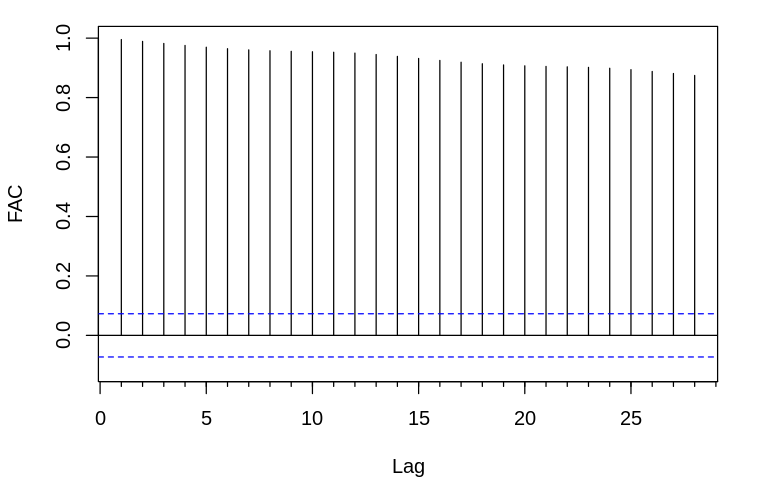
\includegraphics[width=.6\linewidth]{images/acf_co2.png}
    \source{Elaborado pelo autor a partir de \citeonline{co2data}}
\end{figure}

Pela \autoref{fig:correlogramaCo2}  podemos concluir que as  leituras do $CO_2$
apresentam  uma  tendência, e  ainda  por  apresentar todos  valores  positivos
podemos afirmar que  crescerá ao longo do tempo. Como  a série possui tendência
temos  de  fazer  uma   diferenciação,  como  disposto  na  \autoref{sec:diff},
para  remoção  dessa componente,  vemos  a  série  após essa  diferenciação  na
\autoref{fig:co2diff} e o  correlograma após a diferenciação pode  ser visto na
\autoref{fig:acfco2diff}, nesse  novo gráfico é  percebido que a  componente da
tendência foi  realmente removida  após uma  diferenciação, tornando  visível a
componente sazonal, vemos  isso pela alternância das  correlações observadas no
correlograma.

\begin{figure}
    \centering
    \caption{Gráfico de função de autocorrelação da diferenciação da série de
        $CO_2$}\label{fig:acfco2diff}
    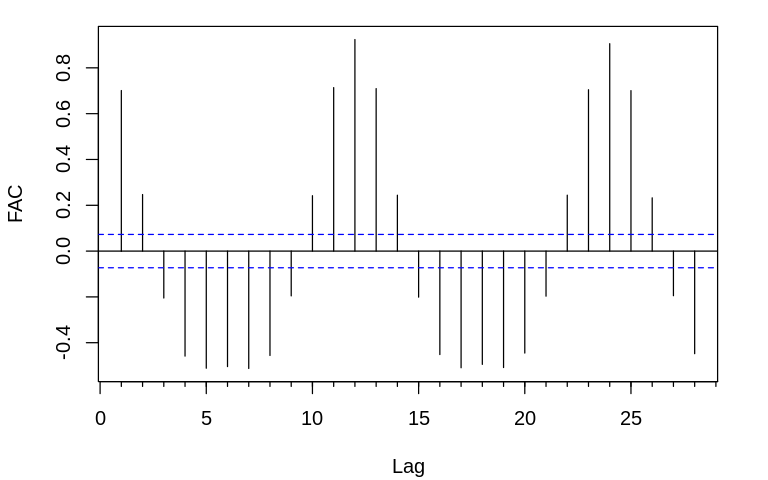
\includegraphics[width=.6\linewidth]{images/acf_co2_diff.png}
    \source{Elaborado pelo autor a partir de \citeonline{co2data}}
\end{figure}

% TODO: Citar as seções nas quais o correlograma é apresentada em outros
%cenários

\subsection{ARIMA}

O modelo ARIMA já introduzido na seção anterior possui três parâmetros
essenciais $(p,q,d)$ sendo $p$ repensável por definir o numero de observações
considerados no processo auto regressivo, $q$ o numero de diferenciações
necessárias para a remoção da tendencia e $d$ o numero de termos no processo de
medias móveis.

\subsubsection{AR --- Processo auto regressivo}

% TODO Melhorar descrição da forma que é encontrado os coeficientes e a
% utilização do ACF e PACF para identificação do p

Segundo  \citeonline{ehlers}  um  processo  $X_t$  é  chamado  auto  regressivo
de   ordem   $p$,   ou   $AR(p)$,   quando   temos   $X_t$   dado   segundo   a
\autoref{eq:aregressivo}.

\begin{equation}
    \label{eq:aregressivo}
    X_t = \alpha_1X_{t-1}+\epsilon_t
\end{equation}

Como observado  na \autoref{eq:aregressivo}  é um modelo  útil se  for razoável
assumir que o  valor atual depende somente de seus  antecessores imediatos mais
um erro aleatório.

\subsubsection{MA --- Processo de médias móveis}

% TODO Melhorar descrição da forma que é encontrado os coeficientes e a
% utilização do ACF e PACF para identificação do q

Segundo \citeonline{timeseriesExample} o processo de  médias móveis é dado como
a média  dos termos passados  e correntes  e pode ser  descrito matematicamente
segunda a \autoref{eq:pmediasmoveis}.

\begin{equation}
    \label{eq:pmediasmoveis}
    X_t = \epsilon_t - \theta_1\epsilon_{t-1} - \theta_2\epsilon_{t-2} - \theta_{q}\epsilon_{t-q}
\end{equation}

Onde os valores de $\theta$ serão dados após análise da série.

\subsubsection{ARMA --- Modelo misto}

Combinando o  processo AR e MA  podemos obter um modelo  extremamente útil para
descrever  séries temporais.  E a  junção dos  modelos pode  ser expressa  pela
\autoref{eq:arma}.

\begin{equation}
    \label{eq:arma}
    X_t = \mu + \sum_{j=-q}^{q}\sum_{i = 1}^{p} \phi{}x_{t-i}+\epsilon_t+\sum{i = 0}{q}\theta_i\epsilon_{t-i}
\end{equation}

\subsubsection{Integração}

Em  casos  que a  série  analisada  apresenta  não estacionariedade  segundo  a
definição dada  na \autoref{sec:estacionaria}, é necessário  a transformação em
uma  série  estacionaria,  isso  pode ser  facilmente  realizado  utilizando  o
método  descrito  na  \autoref{sec:diferenciacao},  assim  podemos  aplicar  de
forma  adequada o  procedimento  de \citeonline{box}  para  produzir um  modelo
probabilístico que poderá ser utilizado na atividade de previsão da série.

% TODO Referencias??
Normalmente  uma diferenciação  é suficiente  para remover  a tendencia  de uma
série  e a  transformar em  uma série  estacionária, entretanto  em séries  que
apresentem a componente  sazonal pode vir a ser necessária  a aplicação de duas
ou  mais  diferenciações  e  em  casos da  aplicação  de  modelos  SARIMA  essa
diferenciação é aplicada com uma distância  $l$, com esse valor sendo dado pela
sazonalidade da série.

\subsection{Seleção do modelo}

De  acordo com  \citeonline{box} a  identificação do  modelo pode  ser feita  a
partir da análise gráfica  da FAC e FACP, podendo contar com  a ajuda de outros
testes para validação da estacionariedade da série.

% FIXME Corrigir inicio
O modo que  \citeonline{box} desenvolveu análise o  comportamento da correlação
de forma que  para identificar a ordem  do AR, $p$, é suficiente  analisar se o
gráfico do FAC  apresenta decaimento exponencial e FACP apresenta  uma quebra a
partir do elemento $p$  do gráfico. Já a identificação da  ordem do processo de
médias móveis  é feita de modo  análogo, porem o  $q$ é dado pela  elemento que
apresenta  a quebra  no gráfico  do FACP  enquanto o  gráfico do  FAC apresenta
decaimento exponencial.

Se não for  possível identificar a série a partir  deste procedimento, pode ser
que a série apresente tendencia ou sazonalidade. No caso de existir tendência é
necessária a realização  de uma ou mais diferenciações na  série, com essa nova
série agora estacionaria é refeito as verificações e determinadas as ordens.

No caso acima o  modelo obtido ou é da forma $AR(p)$ ou  $MA(q)$ porem em casos
de modelos híbridos ambas funções  devem apresentar comportamento de decaimento
a partir do $p$ para o FAC e $q$ para FACP\@. Na \autoref{tab:facpacf} podemos
temos essa seleção de forma sumarizada.


\begin{table}[ht]
    \centering
    \caption{Modelo conforme FAC e FACP}\label{tab:facpacf}
    \begin{tabular}{l l l}
        \multicolumn{1}{c}{Modelo} & \multicolumn{1}{c}{FAC} & \multicolumn{1}{c}{FACP} \\
        \toprule
        Série aleatória  & 0                          & 0                      \\
        AR (1)           & decaimento exponencial     & 0, $k$ > 2             \\
        AR (p)           & decaimento para zero       & 0, $k$ > $p$           \\
        MA (1)           & 0                          & decaimento oscilatório \\
        ARMA (p, q)      & decaimento a partir de $p$ & decaimento a partir de $q$
    \end{tabular}
    \source{\citeonline{ehlers}}
\end{table}

% FIXME Repetitivo
Porem, segundo  \citeonline{vinay} essa  forma nos  fornece modelos  que servem
somente  como uma  boa aproximação,  para determinação  de um  modelo realmente
eficiente  pode  ser necessário  a  execução  de  um  grande número  de  testes
exaustivos e selecionar  aquele modelo que apresente modelo  parcimonioso e que
gere  um  bom resultado,  para  isso  podemos  comparar  os diversos  testes  a
partir  da  minimização  do  critério  de  informação  de  Akaike  que  segundo
\citeonline{ehlers}  propicia  a identificação  de  um  modelo ao  mesmo  tempo
parcimonioso e representativo para a série analisada.

\subsection{Determinação dos coeficientes}

Por fim, para completa construção do modelo apresentado na \autoref{eq:arima} é
necessária  a  obtenção  dos  coeficientes tanto  do  processo  autorregressivo
tanto  do de  médias móveis.  Para essa  tarefa segundo \citeonline{yinay} é
comum a utilização do estimador de \textit{likelihood}, ou mais precisamente a
maximação da função de \textit{likelihood}.

Essa  maximização   é  descrita   por  \citeonline{statiticalML}   da  seguinte
forma.  Considerando  uma função  $q(x;\theta)$  que  nos retorna  a  densidade
probabilística de uma entrada $x$ com um conjunto de parâmetros a ser otimizado
$\theta$ de dimensão $b$, o objetivo é a maximização da \autoref{eq:likelihood}
que nos retorna a capacidade dos parâmetros em aproximar a série.

\begin{equation}\label{eq:likelihood}
    L(\theta) = \prod_{i=1}^{n}{q(x_i;\theta)}
\end{equation}

\section{Aprendizado de Máquina}

Computadores se utilizam de algorítimos  para realizar processamento de dados e
na  solução  de  problemas,  porem, para  determinados  problemas  não  existem
algoritmos.  Por  exemplo a  classificação  de  um  e-mail como  indesejado  ou
legitimo  pode se  tornar  um problema  muito complexo  para  se determinar  um
algorítimo  capaz  de realizar  a  correta  identificação, considerando  que  a
definição de \textit{spam} pode variar com o tempo e usuário.

Conforme \citeonline{ethem} quando  temos tarefas como a  identificação de spam
apresentada que  não apresenta solução  evidente, porem, permite  identificar a
existência  de um  padrão no  conjunto de  dados, pode-se  aplicar técnicas  de
mineração  de dados  em volumes  de dados  massivos em  buscas desses  padrões.
Entretanto para classificarmos  esse sistema como inteligente  não é suficiente
ser capaz de concluir padrões de uma base, precisamos que este ainda seja capaz
de se adaptar a mudanças e aprender com isso.

Considerando  a definição  apresentado  e segundo  \citeonline{machineLearning}
aprendizado de máquina  é descrito como a habilidade  de algorítimos reconhecer
padrões  em um  conjunto  de  dados. Essa  detecção  de  padrões permitem,  por
exemplo, a realização das seguintes atividades.
\begin{itemize}
    \item Classificação\\
        Realiza  o  mapeamento  de  uma   entrada  a  uma  categoria,  como  no
        exemplo  na  classificação  dos   números,  apresentada  no  início  da
        seção.  Podemos   encontrar  ainda  exemplos  do   uso  de  aprendizado
        de  máquina  para  classificação  em diversos  outros  trabalhos, sendo
        aplicado desde a classificação de texto à identificação de riscos em
        aplicações financeiras.
    \item Regressão\\
        Já  a  tarefa de  regressão  é  aplicada  quando precisamos  mapear  um
        conjunto  de valores  a  uma  saída em  $  \mathbb{R}  $, por  exemplo,
        \citeonline{regressao}   utilizou   redes  neurais   artificiais   para
        encontrar um  modelo que  permitisse a  previsão da  demanda de  uso de
        energia elétrica,  mapeando o  carga atual  e informações  climáticas a
        carga futura.
\end{itemize}

Um  exemplo   de  uso  de   aprendizado  de   máquina  é  a   identificação  de
caracteres  numéricos   escritos  a  mão,   esse  exemplo  é   apresentado  por
\citeonline{machineLearning} é  descrito como  um problema de  classificação na
qual uma imagem  de dimensões $28 \times  28$ pixeis é dada como  entrada em um
sistema e este deve atribuir uma classificação que descreve qual o número que a
figura representa,  um conjunto  de exemplo  dessas imagens  pode ser  visto na
\autoref{fig:numeroClassi}.

\begin{figure}
    \centering
    \caption{Exemplo de entrada para o algorítimo de
        classificação}\label{fig:numeroClassi}
    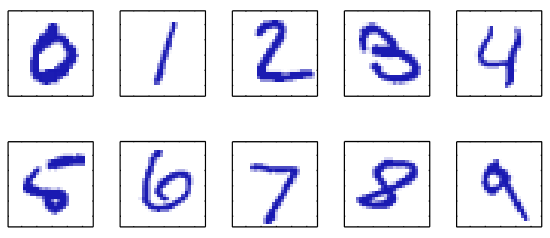
\includegraphics[width=.5\linewidth]{images/numeroClassificacao.png}
    \source{\citeonline{machineLearning}}
\end{figure}

No exemplo apresentado na  \autoref{fig:numeroClassi} podemos entender a tarefa
como  um sistema  onde $x$  é a  entrada  e $\hat{y}$  é a  saída do  sistemas.
Matematicamente  podemos expressar  da  forma vista  na \autoref{eq:sisCla}.  A
saída será na forma  de um conjunto de números variando de 0  a 1 expressando a
probabilidade  de  $x$ pertencer  à  classe  $\hat{y}_i$  onde  $i$ é  o  valor
expressado na imagem.

\begin{equation}
    \label{eq:sisCla}
    f(x) = \hat{y}
\end{equation}

\subsection{Redes Neurais artificiais}

Segundo  \citeonline{haykin2009}  a pesquisa  em  redes  neurais artificiais  é
motivada pelo entendimento que o cérebro  humano realiza o processamento de uma
forma  completamente diferente  dos computadores  convencionais. Essa  forma de
realizar  o processamento  realizado  pelo cérebro  é  altamente complexa,  não
linear e altamente paralela. A unidade de processamento e organização básica de
um cérebro são  os neurônios, o autor ainda lhe  confere superior capacidade na
realização de  tarefas como  reconhecimento de padrões  do que  os computadores
digitais.

Os animais  já nascem com  o cérebro possuindo  certa estruturas que  estes vão
precisar  durante sua  vida,  porem este  é concebido  ainda  de maneira  muito
plastica, ou seja,  possuindo ainda a capacidade de na  fase de aprendizado ser
capaz de se adaptar ao contexto em  que vai se desenvolver. Este mesmo conceito
de  plasticidade  também será  utilizado  para  a  modelagem de  redes  neurais
artificiais~\cite{haykin2009}.

\subsubsection{\textit{Perceptron}}

Como  já  colocado, as  redes  neurais  possuem  o  neurônio como  elemento  de
processamento,  este em  redes artificiais  associamos ao  \textit{perceptron},
descrito primeiramente  por Rosenblatt em  1962, e  tem sua função  definida em
\autoref{eq:perceptron}  sendo  dado  como  a  soma  ponderada  por  $w_i$  das
entradas,  $x_i$. Visualmente  o \textit{perceptron}  é representado  segundo a
\autoref{fig:perceptron}.

\begin{equation}\label{eq:perceptron}
    v(x) = \sum_{i=1}^{m}{w_i  x_i + b}
\end{equation}

\begin{figure}[ht]
    \centering
    \caption{Representação gráfica de um \textit{perceptron}}\label{fig:perceptron}
    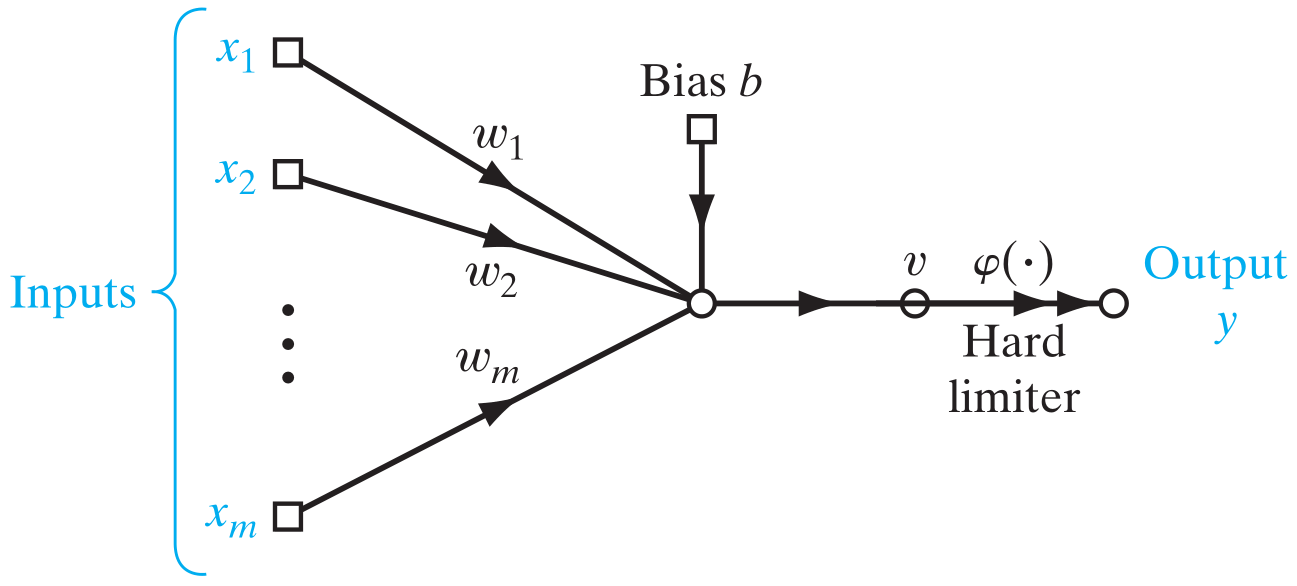
\includegraphics[width=.5\linewidth]{images/perceptron.png}
    \source{\citeonline{haykin2009}}
\end{figure}

Após  a soma  ponderada é  aplicada ao  resultado $v$  uma função  de ativação,
classicamente essa função é dado como uma função de limiar, ou seja, se o valor
resultado da soma  ponderado for maior que um valor  determinado o resultado do
processamento do neurônio artificial é 1 caso contrario 0~\cite{knight}.

Um exemplo  dessa função de limiar  é dada da forma  da \autoref{eq:funLimiar},
nesse exemplo a função resulta em 1 quando  o valor do perceptron é maior que 0
e 0 quando menor.

\begin{equation}
    \label{eq:funLimiar}
    o(v) = \left\{
        \begin{array}{lr}
            1 & :se\  v(x) > 0\\
            0 & :se\  v(x) < 0
        \end{array}
    \right.
\end{equation}

Ainda segundo  \citeonline{knight} o  \textit{perceptron} se  caracteriza pelos
pesos  e pela  definição  do valor  da  função  de ativação,  e  o processo  de
aprendizagem se caracteriza pela modificação desses pesos e valores.

Porem a  utilização de  sistemas simples com  somente um  \textit{perceptron} é
insuficiente na solução de muitos problemas que segundo \citeonline{knight} ele
sozinho  é incapaz  de traçar  hiperplanos  capazes de  resolver problemas  não
lineares, no  exemplo apresentado  por \citeonline{knight} neste  é apresentado
que  enquanto um  neurônio  artificial  é capaz  de  reproduzir corretamente  o
comportamento de um porta logica E ou OU este não consegue sintetizar uma porta
OU-exclusivo, com isso é definido um limite ao \textit{perceptron} já que este
é incapaz de resolver algumas classes de problemas.

\subsubsection{Redes neurais \textit{feedforward}}

Ainda considerando  a incapacidade do  \textit{perceptron} de uma  única camada
modelar algumas superfícies \citeonline{knight} apresenta que se empregado mais
de  uma  camada seremos  capazes  então  de  representar esses  problemas  mais
complexos. A essa arquitetura de organização de neurônios se dá o nome de redes
neurais de  múltiplas camadas, e quando  a alimentação é na  direção da entrada
para a saída será classificada também como \textit{feedforward}.

Podemos  entender  uma  rede  neural   de  múltiplas  camadas  em  três  partes
essenciais, a camada  de entrada, a escondida  e por último a  camada de saída.
Sendo a camada  de entrada aquela que recebe as  características do conjunto de
dados. O nome  de \textit{feedforward} é dado devido a  entrada ser apresentada
primeiramente a camada  de entrada e as  ativações fluírem até a  saída. Logo o
resultado da  rede será encontrado  na camada de saída  após passar por  toda a
rede  em uma  única direção.  Visualmente podemos  expressar a  rede segundo  a
\autoref{fig:neuralNetwork}.

\begin{figure}[ht]
    \centering
    \caption{Representação da ligação entre \textit{perceptron} em uma rede
    neural}\label{fig:neuralNetwork}
    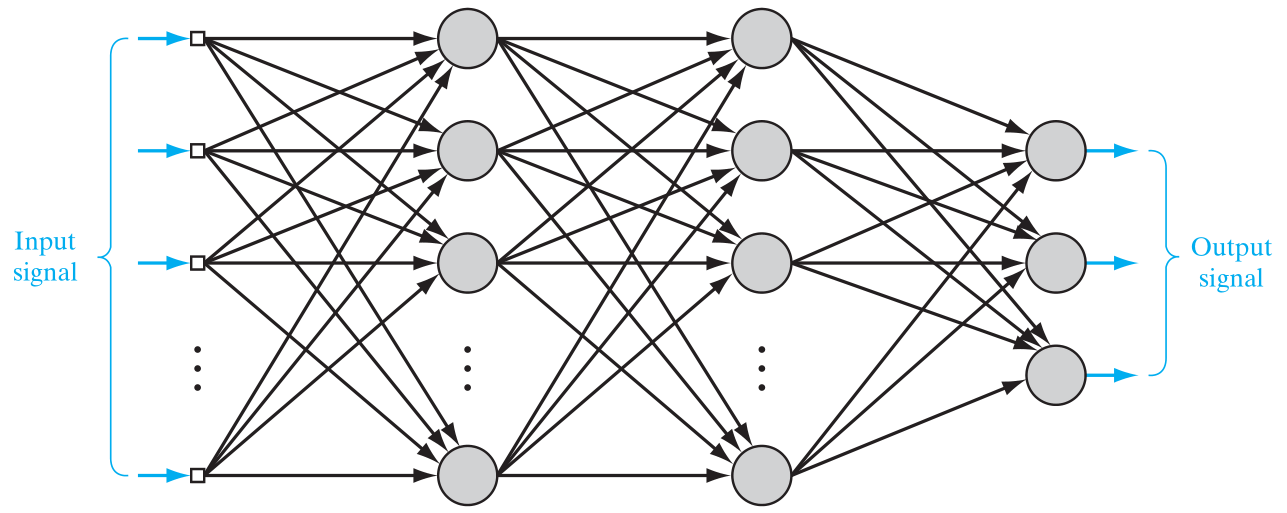
\includegraphics[width=.5\linewidth]{images/neuralNetwork.png}
    \source{\citeonline{haykin2009}}
\end{figure}

Sendo os  parâmetros a  serem definidos  em uma rede  neural somente  os pesos,
$w_i$, definimos que  estes serão inicializados como  valores aleatórios, sendo
reajustados uma vez a cada passagem do aprendizado.

Para avaliação dos  pesos é necessário utilizar uma função  de calculo do erro,
como este trabalho consiste na realização regressão o calculo do erro será dado
pela função de erro absoluto médio conforme \autoref{eq:mae}.

\begin{equation}\label{eq:mae}
    MAE = \frac{1}{n}\sum_{i=1}^{n}{|(Y_i - \hat{Y}_i)|}
\end{equation}

\subsubsection{Retro propagação}

A atualização  dos pesos ocorre  a cada iteração  sobre os valores  de entrada,
assim,  suas  saídas  são  comparadas  com  os  valores  reais  e  computado  o
valor  do erro.  Tendo os  valores  dos erros,  $L$,  esse valor  é aplicado  a
\autoref{eq:backpropagation} e  então os pesos  da rede neural  são atualizados
para a  nova iteração,  sendo aplicado  uma taxa  de aprendizado,  $\alpha$, ao
valor que será corrigido os pesos.

\begin{equation}\label{eq:backpropagation}
    w_{n+1} = w_n - \alpha \frac{\partial L(x,w_t)}{\partial w_t}
\end{equation}

\subsubsection{Avaliação e seleção do modelo}

Após  o treinamento  do  modelo temos  de  avaliar a  capacidade  do modelo  de
generalizar  para  dados  ainda  não  apresentados a  eles,  esse  conceito  de
generalização  é descrito  por \citeonline{haykin2009}  como um  dos principais
objetivos de um modelo neural.

Para avaliarmos a capacidade de generalização normalmente é separado uma porção
dos  dados, normalmente  em uma  proporção de  30\%, assim  durante a  etapa de
treinamento serão  utilizados a porção  maior dos dados  e após o  modelo estar
treinado  é verificado  a qualidade  utilizando a  função de  erro já  definida
anteriormente mas agora no conjunto de teste.

Já  que  durante  a  etapa  de  aprendizado  o  modelo  só  obterá  informações
do  conjunto  de   trinamento  se  faz  necessário   algumas  estrategias  para
impedir  que  o  modelo  se  especialize no  conjunto,  essa  especialização  é
conhecida por  \textit{overfit}, isto pode  causar a incapacidade do  modelo em
prever  corretamente  os  dados  que  ainda não  foram  lhe  apresentado.  Para
impedir  isto  podemos  realizar   os  seguintes  procedimentos  descritos  por
\citeonline{deepLearning}.

\begin{enumerate}
    \item Validação cruzada\\
        O conjunto de dados é divido em sub conjuntos, \textit{folds}, e a rede
        neural é treinada  utilizando $k-1$ \textit{folds}, sendo  $k$ o número
        total de conjuntos  criados, e o modelo é validado  no conjunto deixado
        de  fora do  treinamento.  Ocorrerá  ainda a  mudança  do conjunto  que
        servirá para validação, assim impediremos  que a rede se especialize em
        um conjunto  especifico. Na \autoref{fig:crosvalidation} o  conjunto de
        entrada é dividido  em três \textit{folds} e o  treinamento é realizado
        nas três divisões  criadas, sendo os conjuntos em  azul utilizados para
        treinamento e aqueles em vermelho utilizados para avaliar o modelo, e o
        modelo  é  avaliado  conforme  um  método, $L_{cv}$,  que  reúna  os  a
        avaliação de todos, $L = L_{cv}(L_1, L_2, L_3)$.

        \begin{figure}[ht]
            \centering
            \caption{Divisão da entrada em três\textit{folds}}\label{fig:crosvalidation}
            \includegraphics[width=.5\linewidth]{images/cross_validation.png}
            \source{Elaborado pelo autor}
        \end{figure}

    \item Regularização\\
        Tem  como objetivo  manter os  pesos do  modelo baixos.  O procedimento
        consiste  em alterar  a função  do erro  adicionando a  ela o  custo do
        pesos, isso é  feito conforme a \autoref{eq:regL1}, sendo  $L$ a função
        de perda anterior e $L_{reg}$ a  regularizada, $w$ é os pesos do modelo
        e $\lambda$  é a taxa de  regularização, se selecionado um  valor muito
        alto os  pesos tenderão a  $0$ e o efeito  prático será o  contrario ao
        desejado  e o  modelo passará  a ser  incapaz de  representar também  o
        conjunto de entrada.

        \begin{equation}\label{eq:regL1}
            L_{reg} = L + \lambda \sum{|w|}
        \end{equation}
\end{enumerate}

Como  já  apresentada  existem  diversas definições  a  serem  realizadas  para
produção  do  modelo que  contemple  os  requisitos  do modelo.  Podemos  então
realizar testes nesses diversos modelos  possíveis e escolher aquele que melhor
se adeque segundo a função de  erro definida, esse procedimento é conhecido por
busca em grade,  realizando a avaliação do modelo para  todas as combinações de
parâmetros definidos na grade.

\chapter{Desenvolvimento}\label{chap:desenv}
Como colocado na \autoref{sec:seriesTemporais} a capacidade de se prever séries
temporais tem  grande importância,  e uma  de suas  principais aplicações  é na
previsão  de indicadores  econômicos, como  o S\&P500,  um índice  mantido pela
Standard \& Poor's desde 1923, indexando os  valores de 500 ativos em bolsas de
valores e  servindo como um indicador  geral do comportamento do  mercado. Logo
foi obtido os dados do S\&P500 para comparar os modelos apresentados e observar
as previsões que estes foram capazes de realizar considerando essa série.

Para   podermos   compreender   o   comportamento  dos   modelos   com   outros
tipos   de  séries   foi  também   selecionada  a   série  já   apresentado  na
\autoref{sec:seriesTemporais} que contem os dados  da concentração de $CO_2$ na
atmosfera. A  importância de  avaliar comportamento  com essa  série se  dá por
conta do  se diferenciar da  série econômica  por ter sazonalidade  e tendência
muito mais claras.

Durante  toda  a  etapa  de   desenvolvimento  foi  utilizada  a  linguagem  de
programação python em conjunto com jupyter  para a análise das séries, produção
dos modelos  e avaliação. Especificamente  para os modelos  probabilísticos foi
utilizado a  biblioteca statsmodels\footnote{\url{https://www.statsmodels.org}}
e  tensorflow\footnote{\url{https://www.tensorflow.org/}}  para os  modelos  de
aprendizado de máquina.  Além delas foram utilizadas a  biblioteca seaborn para
produção  dos gráficos  e  pandas em  conjunto com  numpy  e scikit-learn  para
importar e realizar as modificações necessárias dos dados.

As observações das séries podem ser obtidas
online\footnote{\url{https://datahub.io/core/s-and-p-500}}\footnote{\url{https://datahub.io/core/co2-ppm}}.
Na   \autoref{fig:sp500}  e   \autoref{fig:co2}  observamos   a  plotagem   das
observações  do   índice  S\&P500  e   as  leituras  do  $CO_2$   na  atmosfera
respectivamente.

\begin{figure}[ht]
    \centering
    \caption{Gráfico das observações do índice S\&P500}\label{fig:sp500}
    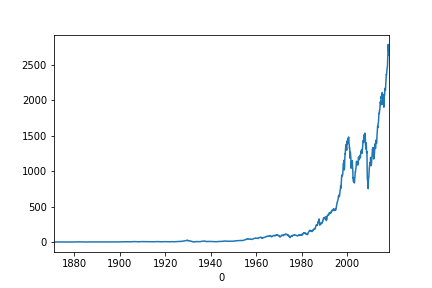
\includegraphics[width=.5\linewidth]{images/sp500.png}
    \source{Elaborado pelo autor}
\end{figure}

A  divisão do  conjunto  de treino  e  teste  foi realizado  de  maneira a  ser
utilizado 70\% dos dados durante o treinamento e 30\% durante a validação.

Após a análise da série foi encontrado os modelos que mais se adequem as séries
apresentadas e validada  a capacidade deste modelo prever um  dia adiante. Para
tornar a  comparação justa  foi definido algumas  considerações aos  modelos de
aprendizado, como a quantidade de observações consideradas para a previsão.

\section{Análise da série}

Seguindo as etapas para construção do modelo foi realizada a análise dos dados.
O  objetivo  era identificar  as  características  da  série,  como se  esta  é
estacionaria, e quanto  a existência de tendencia e  sazonalidade, sendo também
já realizada a remoção de \textit{outliers} que possam atrapalhar na construção
do modelo.

Já   na   análise   dos   gráficos  das   séries   na   \autoref{fig:sp500}   e
\autoref{fig:co2} fica  evidente o comportamento  não estacionário de  ambas as
séries, conclui-se  isso segundo  os critérios  definidos anteriormente.  Já se
aproveita para perceber a existência clara de tendência em ambos conjuntos.

Para  tornar  a  série  estacionaria é  necessário  realizar  inicialmente  uma
diferenciação.  Na \autoref{fig:co2diff}  temos  a  primeira diferenciação  das
leituras de $CO_2$, já para  a série financeira temos a \autoref{fig:sp500diff}
em sua primeira  diferenciação. Pela observação podemos concluir  que uma única
diferenciação foi suficiente em ambos os casos.

\begin{figure}[ht]
    \centering
    \caption{Primeira diferenciação dos dados do SP500}\label{fig:sp500diff}
    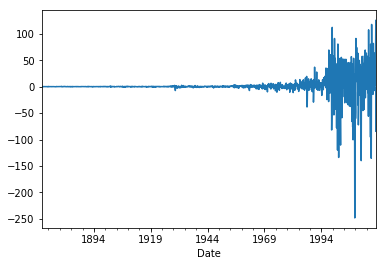
\includegraphics[width=.5\linewidth]{images/sp500diff.png}
    \source{Elaborado pelo autor}
\end{figure}

Quanto a sazonalidade é evidente a sua existência nas leituras de $CO_2$, sendo
esta anual e tendo que as leituras são mensais podemos dizer que a sazonalidade
se repete a cada  12 leituras, no entanto, tal constatação não  é tão clara nos
índices da  Standard \&  Poor sendo  necessários outros  métodos que  não foram
discutidos nesse trabalho para a sua definição.

Tendo sido realizada  a análise pode-se estimar que os  modelos ARMA não seriam
suficientes  e que  seria a  necessária  utilização do  modelo integrado,  alem
disso, seria adequado a aplicação do modelo com suporte a sazonalidade, SARIMA,
à série  contendo leituras  de $CO_2$,  no entanto,  por conta  da complexidade
adicional este não fez parte do desenvolvimento desse trabalho.

\section{Definição do modelo probabilístico}

%TODO Definição do modelo CO2

Compreendido  o  comportamento  da  série  se definiu  a  correlação  entre  as
observações para possibilitar a construção  do modelo probabilístico, usando do
gráfico  da  função  de autocorrelação  apresentado  na  \autoref{fig:sp500acf}
em   conjunto  com   o  gráfico   da  função   de  autocorrelação   parcial  da
\autoref{fig:sp500pacf} foi compreendido seguindo  o modelo de \citeonline{box}
que por conta  de ambos gráficos apresentarem somente um  valor significativo o
modelo probabilístico escolhido  para representar a série S\&P500  foi o modelo
ARIMA(1,1,1), sendo este hibrido do modelo AR(1) e MA(1) com uma integração.

\begin{figure}[ht]
    \centering
    \caption{Gráfico dos 40 primeiros elementos da função de autocorrelação da
    série S\&P500}\label{fig:sp500acf}
    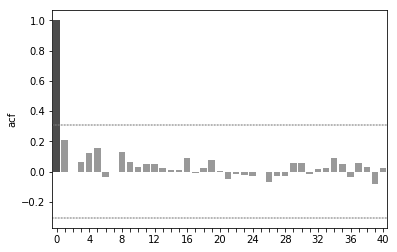
\includegraphics[width=.5\linewidth]{images/sp500acf.png}
    \source{Elaborado pelo autor}
\end{figure}

\begin{figure}[ht]
    \centering
    \caption{Gráfico  dos 40  primeiros elementos  da função  de autocorrelação
    parcial da série S\&P500}\label{fig:sp500pacf}
    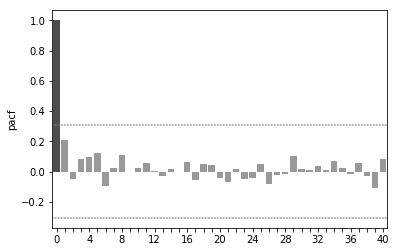
\includegraphics[width=.5\linewidth]{images/sp500pacf.png}
    \source{Elaborado pelo autor}
\end{figure}

\section{Definição do modelo utilizando aprendizado de máquina}

Já para  o desenvolvimento do modelo  neural não foi necessária  uma observação
profunda da  série, no entanto,  exigiu uma parametrização muito  mais complexa
do  modelo,  observando como  o  modelo  convergia considerando  os  parâmetros
escolhidos e realizando  uma busca em grade extensiva para  encontrar um modelo
com boa capacidade representativa.

Antes da etapa de parametrização  foram realizadas alguns pré-processamentos, o
primeiro foi  em vista  de escalar a  série para o  intervalo 0  e 1, já  que a
função  de  ativação  utilizada  tem  esse  intervalo  como  saída.  Para  isso
foi  utilizado o  método de  \textit{MinMaxScaler} da  biblioteca sklearn,  que
matematicamente pode ser representado  como visto na \autoref{eq:minmaxscaler},
sendo $MAX$ e  $MIN$ o maior e  menor valor respectivamente no  conjunto após o
procedimento.

\begin{align}\label{eq:minmaxscaler}
    &X_{std} = \frac{X - \min X}{\max X-\min X}\\
    &X_{scaled} = X_{std} * (MAX-MIN)+MIN
\end{align}

Na \autoref{tab:gridsearch} observamos todos os parâmetros testados na busca em
largura.

\begin{table}[ht]
\centering
\caption{Possibilidades dos parâmetros da busca em grade}\label{tab:gridsearch}
\begin{tabular}{l l}
\multicolumn{1}{c}{Parâmetro}        & \multicolumn{1}{c}{Possibilidades}  \\
    \toprule
    Número de camadas                & 1 \ldots 4                          \\
    Número de unidades por camada    & 1 \ldots 20                         \\
    $\lambda$ regularização          & 0.00001 \ldots 0.0001               \\
    Função de ativação               & $relu$, $sigmoid$                   \\
    Função de perda                  & MSE, MAE                            \\
    Iterações                        & 20 \ldots 500
\end{tabular}
\source{Elaborado pelo autor}
\end{table}

Uma característica que foi logo  observada nas primeiras execuções anteriores a
aplicação  da regularização  foi o  rápido \textit{overfit}  sobre os  dados de
treinamento como  visto na \autoref{fig:sp500_overfit}, mesmo  sendo aplicada a
validação  cruzada, e  ainda como  visto na  \autoref{fig:iter_sp500_overfit} a
especialização para o conjunto de treino foi muito rápida, assim foi aplicada a
regularização e após se tornou frequente  encontrar bons modelos para as séries
observadas.

\begin{figure}[ht]
    \centering
    \caption{Gráfico  da  comparação  do  previsto   e  real  para  o  conjunto
    de   treino   e   teste   para   a   série   de   observações   do   índice
    S\&P500}\label{fig:sp500_overfit}
    \minipage{0.50\linewidth}
        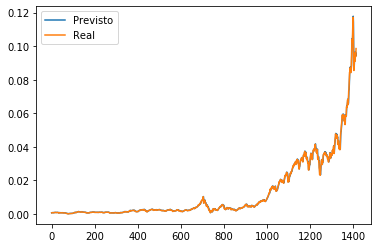
\includegraphics[width=\linewidth]{images/sp500_overfit_train.png}
    \endminipage\hfill
    \minipage{0.50\linewidth}
        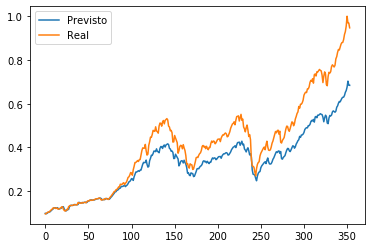
\includegraphics[width=\linewidth]{images/sp500_overfit_test.png}
    \endminipage\hfill
    \source{Elaborado pelo autor}
\end{figure}

\begin{figure}[ht]
    \centering
    \caption{Gráfico da função de perda em  função do números de iterações para
    a série S\&P500}\label{fig:iter_sp500_overfit}
    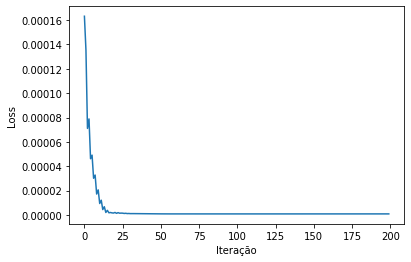
\includegraphics[width=.5\linewidth]{images/sp500_overfit_iter.png}
    \source{Elaborado pelo autor}
\end{figure}

Para os dados  da Standard \& Poors  o modelo selecionado a partir  da busca em
grade  foi com  duas camadas,  sendo a  primeira camada  com 13  neurônios e  a
segunda com somente um  neurônios já que esta é a camada de  saída. A função de
ativação de foi a $relu$ e  o $\lambda$ da regularização ficou como $0.000001$.
A função de  perda selecionada foi $MSE$ e 300  iterações foram suficientes. Já
que  o modelo  probabilístico  tem AR(1)  foi fixado  em  uma única  observação
no passado para a realização da previsão.

\chapter{Resultados}\label{chap:result}

A  partir  dos  modelos  gerados   foram  obtidos  os  resultados  apresentados
na   \autoref{tab:resultadosp500}   e  o   gráfico   do   conjunto  de   testes
comparando  os   resultados  obtidos  com   os  valores  são   apresentados  na
\autoref{fig:comparesp500}.  Observando  os  resultados  é claro  que  os  dois
modelos conseguiram exito  na tarefa de aproximar o comportamento  da série. Em
termos  comparativos o  modelo neural  obtive resultado  um pouco  inferior, na
ordem de $0.6\%$.

\begin{table}[ht]
    \centering
    \caption{Valores do erro para a série S\&P500}\label{tab:resultadosp500}
    \begin{tabular}{ll}
        \multicolumn{1}{c}{Modelo} & \multicolumn{1}{c}{MSE} \\
        \toprule
        MLP                        & 0.0002101               \\
        ARIMA                      & 0.0002088
    \end{tabular}
    \source{Elaborado pelo autor}
\end{table}

\begin{figure}[ht]
    \centering
    \caption{Gráfico comparativo entre os modelos obtidos para a série
    S\&P500}\label{fig:comparesp500}
    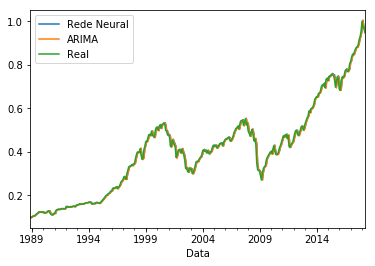
\includegraphics[width=.5\linewidth]{images/sp500_prediction_compare.png}
    \source{Elaborado pelo autor}
\end{figure}

\chapter{Conclusões}\label{chap:concl}

\section{Trabalhos futuros}

\postextual

\bibliography{referencias}

\end{document}
